\chapter{Тестирование и аппробация плагина в Jenkins} \label{ch4}

% не рекомендуется использовать отдельную section <<введение>> после лета 2020 года
%\section{Введение. Сложносоставное название первого параграфа первой главы для~демонстрации переноса слов в содержании} \label{ch1:intro}

В главе описано проведенное тестирование и аппробация плагина:

\begin{enumerate}
	\item Описаны методы тестирования.
	
	\item Проведена аппробация плагина в системе Jenkins.
	
	\item Разработан код тестирования плагина.
	
	
	
\end{enumerate}

\section{Методы тестирования} \label{ch4:sec1}

Тестирование программного обеспечения — обширное понятие, которое включает планирование, проектирование и, собственно, выполнение тестов  \cite{testing}. В процессе CI/CD производится непрерывное тестирование разработанного кода, а также тестирование разработанного приложения. Сам плагин является частью CI/CD процессе, но также требует тестирования корректной работы своей функциональности, тестирование разработанного кода, а также тестирования на сооветсвие исходным требования, которые были предъявлены к разработке в главе 1.

Существует множество методов тестирования и техник тест дизайна, в процесе анализ функциональных требования были отобраны те, которые наиболее релевантны для разработанного плагина Jenkins.

Будет проведено как ручное, так и автоматизированное тестирование плагина. Ручное тестирование поможет выявить нетипичные тест-кейсы, которые не покрываются автоматизированными тестами.

Ручные тесты будут проведены методом черного ящика. Данный метод это процедура получения и выбора тестовых случаев на основе анализа функциональности и технического задания, без применения знаний о внутреннем устройстве системы \cite{blacktest}.

Были составлены следующие тест-кейсы:

\begin{table}
    \centering
    \begin{tabular}{|p{1cm}|p{5cm}|p{9cm}|}
    \hline
        № & Описание & Ожидание  \\ \hline
        1 & Проверка выбранного периода на графике Success Rate (месяц) & Количество  дней соотвествует прошлому месяцу, на каждый день отображены корректные значения процента успешности сборок\\ \hline
        2 & Проверка выбранного периода на графике Build Duration (неделя) с учетом выбора настройки среднего значения и  упавших сборок& Количество  дней 7 в соотвествии со всеми днями недели, на каждый день отображены корректные значения среднего времени продолжительности сборок, учтены упавшие сборки \\ \hline
        3 & Проверка выбранного периода на графике Time Spent in queue (квартал) с учетом выбора настройки среднего значения & Количество  кварталов 4 в соотвествии с кварталами года, на каждый квартал отображены среднии значения проведенного в очереди времени сборок  \\ \hline
        4 & Проверка выбранного периода на графике Test Count (год) с учетом выбора настройки упавших сборок & Количество  месяцев 12 соотвествует прошедшему году, на каждый месяц отображены корректные значения  количества тсетов, с учетом тестов выполненыных на упавших сборках \\ \hline
        5 & Проверка выбранного периода на графике Artifacts Size (день) & Количество  часов 24 соотвествует всем часам прошедшего дня, на каждый час отображены корректные значения размера итоговых артефактов полученного по результатм задания   \\ \hline
        6 & Проверка корректного отображения при выборе периода ALL & Отображены сборки со всего периода прошедшео, информация поделена на равное части   \\ \hline
        7 & Проверка корректного отображения аномальных значений & Отображены номера сборок, возде каждого графика, у которых аномальное значений метрики соотвествующей графику   \\ \hline
        8 & Проверка корректного расчета предугаданной 'следущей' сборки& Метрики предугаданной сборки расчитываются корректно для каждого графика   \\ \hline

    \end{tabular}
\end{table}

В данном случае тест-кейсы были описаны с помощью техники тест-дизайна Матрица трассировки. Если обратиться к определению, то матрица трассировки — двумерная таблица, содержащая соответствие функциональных требований и подготовленных тестовых сценариев \cite{matrixtest}, а на пересечении столюбцов и строк ставится метка, о том, что данное требование покрывается данным тест-кейсом. В случае данной работы из соображений удобства и оптимизации тестовой документации, было принято решение модифицировать матрицу трассировки и совместить с подробным описание в формате чек листа: для оптимизации идет проверка, что каждый тип графика-метрики (Success Rate) корректно себя ведет на определенном периоде (неделя), таким образом не придется проверять, каждый график на каждом пероде при каждой доработке кода продукта.

Данные тест-кейсы оптимизированы, поскольку в соотвествии с пирамидой тестирования \cite{TestPyramid} ручные UI кейсы, находятся в самой верхней ее части и не должны занимать достаточно большое место в системе тестирования. С дрйгой стороны для улучшения покрытия требования, предъявляемых к продукты должны использоваться гораздо в большем объеме unit-тесты, т.е. тесты в которых самые маленькие компоненты системы - модули (модули, классы, методы), индивидуально проверяются на предмет правильной работы \cite{unittest}.

При написание юнит тестов используется метод белого ящика. Данный метод предоставляет тестировщику полное знание тестируемого приложения, включая доступ к исходному коду и проектной документации \cite {whitebox}, т.е. тестирование происходит на основе знания исходного кода, таким образом, юнит тестирование методом белого ящика поможет нам достаточно широко покрыть все модули плагина.

Код юнит тестов приведен в приложении 5.

Также для автоматизации тесстиования UI части плагина, был применен Selenium web driver и язык программирования python. WebDriver управляет браузером, как это делает пользователь, с использованием сервера Selenium \cite{webdriver}. Данные тест-кейсы будут в автоматическом режиме проверять реакцию элементов веб интерфейса на действия пользователя.

Код UI тестов приведен в приложении 6.



 \section{Аппробация плагина} \label{ch4:sec2}
 
 Аппробация плагина будет проводится в системе CI Jenkins для которой и был разработан плагин визуализации. Для того чтобы провести аппробацию плагина на локальном сервере дженкинс, запущенном на локальном или удаленном ПК, потребкется произвести несколько операций. Для начала, нужно будет склонировать репозитоорий с кодом плагина на GitHub, перейти в папку проекта и выполнить \cite{deployplugin} Maven mvn install и скопировать .hpi в папку /plugins/. 
 
 Затем потребуется на запущенном серере дженкинс перейти в Управление Jenkins  и среди доступных плагинов выбрать Build Configuration Statistics, установить, после чего напротив каждой сборки дженкинс в боком меню, откуда можно запустить и отредактировать сборку, появится пункт меню Build Configuration Statistics, при нажатии на которой должны отобразиться все графики с собранной статистикой по метрикам каждого задания в Jenkins. 
 
 Для того чтобы графики отображали какие-то данные, необходимо сначала сгенерировать сборки разной длительности, статусов, с разным количеством тестов и размером артефактов.
 
 В ходе аппробации плагина были сгенерированы следующие сборки.
 
 \begin{figure}[ht!] 
	\center
	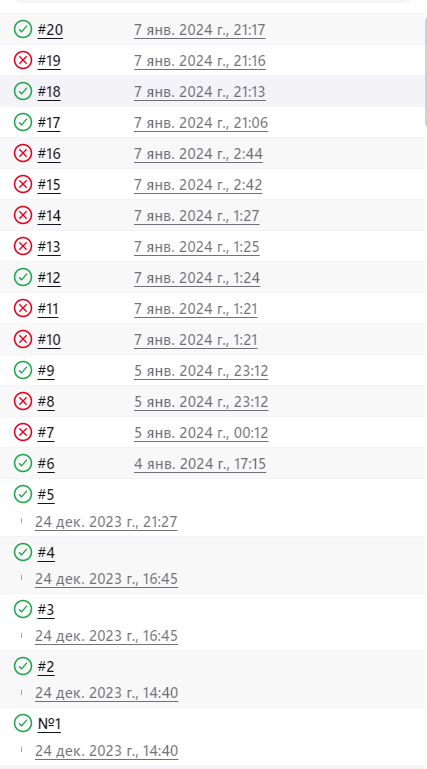
\includegraphics [scale=0.47] {my_folder/images//builds}
	\caption{Сгенерированые сборки} 
	\label{fig:builds}  
\end{figure}


 Среди сборок присутсвуеют, упавшие сборки со специально завышенным временем выполнения.
 
 \begin{figure}[ht!] 
	\center
	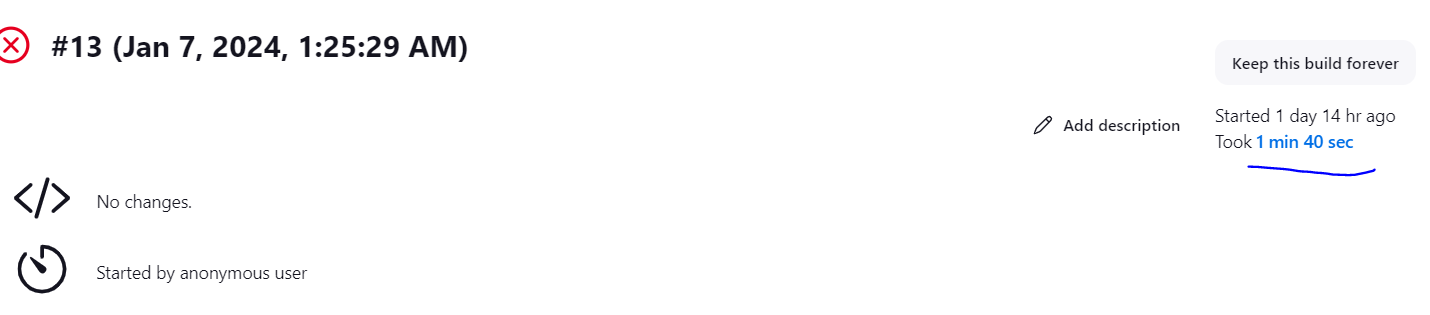
\includegraphics [scale=0.47] {my_folder/images//longBuild}
	\caption{Длинная упавшая сборка} 
	\label{fig:longBuild}  
\end{figure}


А также сборки, с созданными артефактами, часть из которых в статусе успешного выполнения, с короткой продолжительностью.
 
 \begin{figure}[ht!] 
	\center
	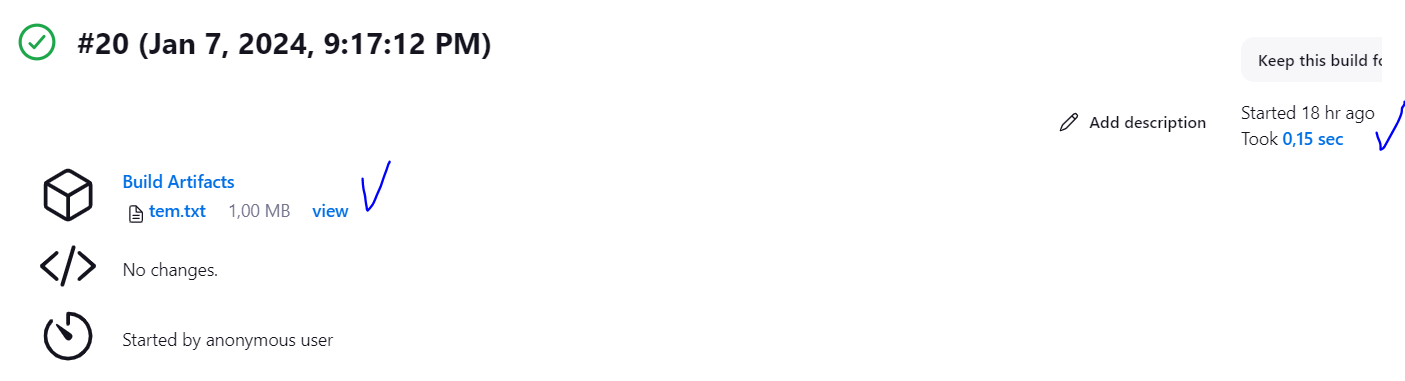
\includegraphics [scale=0.47] {my_folder/images//artifactBuild}
	\caption{Короткая успешная сборка с артефактом} 
	\label{fig:artifactBuild}  
\end{figure}
 
 
\section{Выводы} \label{ch4:sec3}

После проведения этапа аппробации и тестирования плагина визуализации статистики сборок Jenkins можно прийти к выводу, что тестировоние проведено в полном объеме и затронуло разные методы, техники тест-дизайна и соответсвует методологиям и устоявшимся практикам тестирования программного обесечения. Аппробация протестированного плагина, далп понять, что плагин корректно отрабатывает при разных поданных на вход исходных данных и настройках.






%
%

%
%
%\begin{table} [htbp]% Пример оформления таблицы
%	\centering\small
%	\caption{Представление данных для сквозного примера по ВКР \cite{Peskov2004}}%
%	\label{tab:ToyCompare}		
%		\begin{tabular}{|l|l|l|l|l|l|}
%			\hline
%			$G$&$m_1$&$m_2$&$m_3$&$m_4$&$K$\\
%			\hline
%			$g_1$&0&1&1&0&1\\ \hline
%			$g_2$&1&2&0&1&1\\ \hline
%			$g_3$&0&1&0&1&1\\ \hline
%			$g_4$&1&2&1&0&2\\ \hline
%			$g_5$&1&1&0&1&2\\ \hline
%			$g_6$&1&1&1&2&2\\ \hline		
%		\end{tabular}	
%	\normalsize% возвращаем шрифт к нормальному
%\end{table}


% \firef{} от figure reference
% \taref{} от table reference
% \eqref{} от equation reference




